\section{Entrenamiento en la última capa}

En esta sección nos vamos a enfocar en la última capa de red, consideremos la siguiente red de la figura \ref{fig:REDuc}. 

\begin{figure}[H]
 \centering
 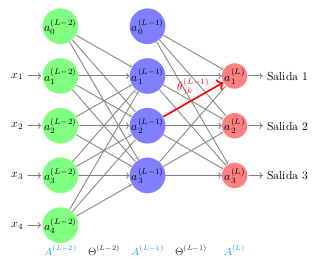
\includegraphics[scale=0.7]{../Figuras/AredNa.png}
 \caption{Red neuronal(entrenamiento última capa.)}
 \label{fig:REDuc}
\end{figure}

Vamos a calcular el gradiente considerando que estamos evaluando a la red para un ejemplar. Una vez que la red tomó los valores de entrada (neuronas en verde) y los evaluó pasando por la capa oculta (neuronas en azul) hasta asignar el ejemplar a una neurona de salida (neuronas en rojo). Lo que la función de error está midiendo es la \textit{distancia} entre lo que obtuvimos en la capa de salida y una colección de etiquetas objetivo, es decir, la clasificación real del ejemplar. 


Entonces por ahora nuestra función de error está actuando solo sobre la capa de salida, pero recordemos que para llegar a la evaluación de cualquiera de las neuronas en la capa de salida, se calculó la activación de la capa oculta y de la capa de entrada. Con los respectivos pesos de cada capa. Entonces podemos decir que los valores obtenidos en la evaluación final dependen directamente de los pesos en cada capa. 


Tomando en cuenta lo anterior, el gradiente lo vamos a calcular capa por capa. Desde la capa de salida hasta la capa de entrada.
Lo primero que tenemos que calcular es como dependió la función de error de los pesos de la capa oculta (azul) que la antecede.


La notación que vamos a usar más adelante va a considerar las neuronas de entrada con el índice $i$, las neuronas de la capa oculta con el índice $j$, y las neuronas de salida con el índice $k$. Así, los pesos que conectan a la neurona $j$ con la neurona $k$, se representan como $\theta_{jk}$. 


Para denotar la capa que estamos haciendo referencia vamos a emplear el superíndice $(L)$ con referencia a last, último en inglés, dado que estamos haciendo los cálculos desde la última capa, hacia atrás, la penúltima capa se va a indicar con $(L-1)$, la anterior de esta como $(L-2)$ y así sucesivamente. Entonces, para referirnos a un peso para la última capa, que conecta a la penúltima capa con la de salida, se escribe como $theta_{jk}^{L-1}$ que es el peso marcado en rojo en la figura \ref{fig:REDuc}.

Usemos la entropía cruzada como función de error, para un ejemplar \ref{entropiaCruzada}:
 \begin{equation}
  J (\Theta) = -\left[\sum_{k=1}^{s_{L}}y_{k}^{(i)} log(\textcolor{blue}{a_{k}^{(L)}}) + (1-y_{k}^{(i)}) log(1 - \textcolor{blue} {a_{k}^{(L)}})  \right] 
  \label{eq:EntropiaCruz}
 \end{equation}
 

 La suma está tomando en cuenta que el ejemplar puede ser clasificado a una de las varias clases a poder asignar $S_{L}$, es decir, el número de neuronas en la capa $L$. Los valores obtenidos de la activación las neuronas están definidos por $a_{k}^{(L)}$, y los deseados por $y_{k}$.
 
 Lo siguiente a hacer es calcular la derivada con respecto a los pesos que conectan la última capa con la penúltima capa, es decir, $\theta_{jk}^{(L-1)}$.
 
 Entonces vamos a calcular la parcial de error con respecto a uno de los pesos de la capa anterior. Así la suma se "va" dado que el peso solo va a afectar a la $k$-esima neurona, quedando solo con la operación que se efectúa en esta, usando la regla de cadena obtenemos lo siguiente:
 
 \begin{equation}
  \dfrac{\partial J}{\partial \theta_{jk}^{L-1}} = - \left[ \dfrac{y_{k}}{a_{k}^{L}} \dfrac{\partial}{\partial\theta_{jk}^{(L-1)}} g(\textcolor{red}{z_{k}}) - \left(\dfrac{1 - y_{k}}{1 - a_{k}^{L}} \right) \dfrac{\partial}{\partial \theta_{jk}^{(L-1)}}g(\textcolor{red}{z_{k}})\right]
 \end{equation}
 
Con:
\begin{equation}
 \textcolor{red}{z_{k}} = \sum_{j'=0}^{S_{L-1}} \theta_{j'k}a_{j'}^{L-1}
\end{equation}

Recodemos que $a_{k}^{(L)}$ está calculado por una función de activación $g(z_{k})$. Donde $z_{k}$ es la suma de las combinaciones lineales de las neuronas conectadas hacia la neurona $k_{n}$. Estos valores son calculados en el algoritmo de propagación hacia adelante. Los escribimos aquí para recodar como está siendo calculada la parcial.

De la derivada de la suma sólo queda $a_{j'} $ con $j' = j$. Siguiendo la regla de la cadena para los términos que nos faltaba nos queda lo siguiente:

\begin{equation}
 \dfrac{\partial J}{\partial \theta_{jk}^{L-1}} =-\left[ \dfrac{y_{k}}{a_{k}^{(L)}} \textcolor{blue}{g'(z_{k})} -\left( \dfrac{1-y_{k}}{1-a_{k}^{(L)}} \right) \textcolor{blue}{g'(z_{k})}\right]a_{j}^{(L)}
\end{equation}

Simplificando, nos queda lo siguiente:

\begin{equation}
 \dfrac{\partial J}{\partial \theta_{jk}^{L-1}} =-\left[ \dfrac{y_{k}(1-a_{k}^{(L)})-a_{k}^{(L)}(1-y_{k})} {a_{k}^{(L)}(1-a_{k}^{(L)})} \right]\textcolor{blue}{g'(z_{k})} a_{j}^{(L)}
\end{equation}

Recordando que la derivada de la sigmoide queda como $g' = g (1 - g)$ tenemos que:
\begin{equation}
 \textcolor{blue}{g'(z_{k})} = a_{k}^{(L)}(1-a_{k}^{(L)})
\end{equation}

Así nos queda como: 
\begin{equation}
 \dfrac{\partial J}{\partial \theta_{jk}^{L-1}} = -\left[ \dfrac{y_{k}- y_{k}a_{k}^{(L)} - a_{k}^{(L)} + a_{k}^{(L)}y_{k} } {a_{k}^{(L)}(1-a_{k}^{(L)})} \right] a_{k}^{(L)}(1-a_{k}^{L}) a_{j}^{(L)}
\end{equation}

Y haciendo un poco de álgebra nos queda como:
\begin{equation}
 \dfrac{\partial J}{\partial \theta_{jk}^{L-1}} =  -a_{j}^{(L-1)})(y_{k}-a_{k}^{(L)})
\end{equation}

Representando a $(y_{k}-a_{k}^{(L)})$ como $\delta_{k}$ nos queda:

\begin{equation}
 \dfrac{\partial J}{\partial \theta_{jk}^{L-1}} =-a_{j}^{(L-1)})\delta_{k}
\end{equation}

Esta última notación con delta se usa pues con esto estamos representando el error que se cometió en la última capa, pues es la diferencia entre lo desado y lo que se obtuvo realmente.

Con esto ya sabemos calcular todas las parciales del error con respecto a los pesos hacia la última capa. En la siguiente sección seguimos con el cálculo para las siguientes capas.
